\section{実装}\label{sec:impl}
本章では、各操作の詳細アルゴリズム及び実装を述べる。
本レポートでは図\ref{fig:question}における頂点ABCDの選定は手動で行うが、頂点EFGHは明示的に選択せず、特徴量マッチングによって暗黙的に行う。この場合、差し替え先画像から適用画像へのホモグラフィ行列は、各ピクセルの対応が分からないため、直接求めることはできない。そこで、テンプレート画像と差し替え先画像の画像サイズを一致させてから、テンプレート画像と適用画像との特徴量マッチングを行うことで、ここから求められるテンプレート画像から適用画像へのホモグラフィ行列が差し替え先画像から適用画像へのホモグラフィ行列に一致する。
このようにして各ピクセルの変換方法が求められるため画像を置換できる。

\subsection{実装環境}
本レポートは次の実行環境で動作させている。
\begin{itemize}
    \item Python 3.7
    \item kivy 1.11.1
    \item OpenCV-python 3.4.2.16
    \item Numpy 1.19.0
\end{itemize}

ここでkivyはGUIのアプリケーションを作成するライブラリであり、
作成したアプリケーションのコントロールやUI処理を担っている。
OpenCVは一部の画像処理アルゴリズムを使用するために導入している。
Numpyは数値計算を目的として導入している。

詳細の実装については\href{https://github.com/SakumaTakuya/cv_finalreport}{GitHubページ}に公開している。
また、アプリケーションのデモンストレーションは添付した「demo.mp4」を参照されたい。

\subsection{テンプレート画像と差し替え先画像の画像サイズ}
\subsubsection{ワーピング処理}
本問題では図\ref{fig:question}(a)の頂点ABCDには任意性があるため、単純なリサイズ処理ではテンプレート画像と差し替え先画像のサイズを一致させることができない。
4点の対応点が与えられるばあにはホモグラフィ行列を用いて変換することが一般的であるが、
本レポートではワーピング処理によって頂点ABCDを矩形に変換する。
変換によって画像にピクセルの抜けが生じないようにするためInverse warpingを実装する。
具体的には以下の図\ref{fig:warp}に示す、
四角形MNOP内の任意の点$\bm{p_1}=(x_1, y_1)$から四角形IJKLの対応する点$\bm{p_0}$を求める。

\begin{figure}[h]
    \centering
    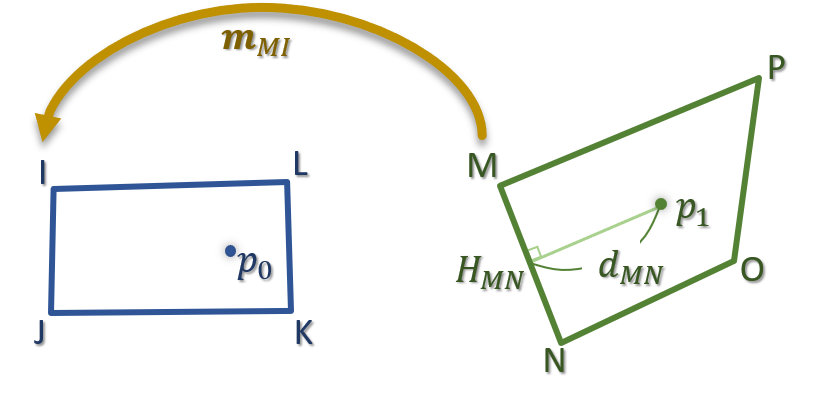
\includegraphics[width=1\linewidth]{fig/warp.png}
    \caption{ワープ処理}
    \label{fig:warp}
\end{figure}


まず、頂点MからIへの移動量を$\bm{m_{MI}} = (dx_{MI}, dy_{MI})$とする。
$\bm{p_1}$から辺MNへの距離及び垂線の足をそれぞれ$d_{MN}$及び$H_{MN}$とする。
また、$\overrightarrow{MH_{MN}}=t_{MN}\overrightarrow{MN}$とすると、
Line-based image warping\cite{}に従って$\bm{x_0}$は以下の式で求める。

\begin{equation}\label{eq:warp}
    \bm{p_1} =  \begin{bmatrix} 
                    x_1 + \left( 1 - \frac{d_{MN}}{d_{MN}+d_{OP}} \right) \left( \left( 1 - t_{MN} \right) dx_{MI} + t_{MN} dx_{NJ} \right) + \frac{d_{MN}}{d_{MN}+d_{OP}} \left( \left( 1 - t_{OP} \right) dx_{PL} + t_{OP} dx_{OK} \right) \\
                    y_1 + \left( 1 - \frac{d_{PM}}{d_{NO}+d_{PM}} \right) \left( \left( 1 - t_{PM} \right) dy_{MI} + t_{PM} dy_{PL} \right) + \frac{d_{PM}}{d_{NO}+d_{PM}} \left( \left( 1 - t_{NO} \right) dy_{NJ} + t_{NO} dy_{OK} \right)
                \end{bmatrix}
\end{equation}

pythonにおける実装は以下のソースコード\ref{py:warp}に示す。

\begin{lstlisting}[caption=ワーピング, label=py:warp]
# 4つの点を指定した影響度でブレンドする関数
def bilinear(
    value,
    left_bottom, 
    right_bottom, 
    left_top, 
    right_top, 
    main_ratio, 
    cross_ratio):
    left_ratio = 1-main_ratio
    right_ratio = main_ratio
    return value \
        + (1-cross_ratio) * (left_bottom * left_ratio + right_bottom * right_ratio) \
        + cross_ratio * (left_top * left_ratio + right_top * right_ratio)


def warp(
    image,
    from_bottom_left,
    from_bottom_right,
    from_top_right,
    from_top_left,
    to_bottom_left,
    to_bottom_right,
    to_top_right,
    to_top_left,
    return_height,
    return_width):

    # 任意の点から各辺への距離(d)とその垂線の足が辺のどのあたりに位置しているかの割合(t)を返す関数を作成
    def td(f, t):
        a = np.array([f, t])
        # fとtの差分 = fを基準としたtへのベクトル
        dif = np.diff(a, axis=0)[0]
        det = np.linalg.det(a)
        sq = dif @ dif
        f = f[:,None,None]
        def ret(x):
            # 直線を表す式:dif[1] * x[0] - dif[0] * x[1] - det=0
            up = (dif[1] * x[0] - dif[0] * x[1] - det)
            r = -up / sq
            # fを基準とした垂線の足へのベクトル
            h_dif = f - np.array([r * dif[1] + x[0], -r * dif[0] + x[1]])
            # ベクトルの大きさの比と点と直線の距離を返戻
            return np.sqrt(np.sum(h_dif**2, axis=0) / sq), (np.abs(up) / np.sqrt(sq))
        return ret
    td_bottom = td(to_bottom_left, to_bottom_right)
    td_top = td(to_top_left, to_top_right)
    td_left = td(to_bottom_left, to_top_left)
    td_right = td(to_bottom_right, to_top_right)

    # 各頂点の移動量を計算
    move_bottom_left = from_bottom_left - to_bottom_left
    move_bottom_right = from_bottom_right - to_bottom_right
    move_top_left = from_top_left - to_top_left
    move_top_right = from_top_right - to_top_right

    h, w, *_ = image.shape

    # 関数の本体:i,jはnp.meshgridで与えられる
    def func(i, j):
        nonlocal to_bottom_left, to_bottom_right, to_top_left, to_top_right
        pos = np.array([i, j])

        # ピクセルが変換先の領域内に含まれているか判定するために外積を求める
        crs_bl = np.cross(
            pos - to_bottom_left[:,None, None],
            to_bottom_right - to_bottom_left,
            axis=0)
        crs_br = np.cross(
            pos - to_bottom_right[:,None, None],
            to_top_right - to_bottom_right, 
            axis=0)
        crs_tr = np.cross(
            pos - to_top_right[:,None, None],
            to_top_left - to_top_right, 
            axis=0)
        crs_tl = np.cross(
            pos - to_top_left[:,None, None],
            to_bottom_left - to_top_left, 
            axis=0)

        # posから各頂点への外積が負なら内部
        mask = np.where(
            (crs_bl < 0) & (crs_br < 0) & (crs_tr < 0) & (crs_tl < 0), 
            1, 0)
        t_bottom, d_bottom = td_bottom(pos)
        t_top, d_top = td_top(pos)
        t_left, d_left = td_left(pos)
        t_right, d_right = td_right(pos)

        t_vert = d_bottom / (d_bottom + d_top)
        t_hori = d_left / (d_left + d_right)

        v = (i\
            +((1 - t_bottom) * move_bottom_left[0] + t_bottom * move_bottom_right[0]) * (1 - t_vert)\
            + ((1 - t_top) * move_top_left[0] + t_top * move_top_right[0]) * t_vert)

        u = (j\
            + ((1 - t_left) * move_bottom_left[1] + t_left * move_top_left[1]) * (1 - t_hori)\
            + ((1 - t_right) * move_bottom_right[1] + t_right * move_top_right[1]) * t_hori)
        
        # バイリニア補完するために隣接ピクセルの影響度を計算
        v_int = v.astype(np.int16)
        u_int = u.astype(np.int16)
        bottom = np.where((v_int < 0) | (v_int > h-2), h-2, v_int)
        left = np.where((u_int < 0) | (u_int > w-2), w-2, u_int)
        top = bottom+1
        right = left+1
        v_ratio = (v - v_int)[:,:,None]
        u_ratio = (u - u_int)[:,:,None]

        return np.where((
                # 内部判定
                (mask == 0) |\
                # 辺の外側に出ていないか判定
                (((t_bottom < 0) | (t_bottom > 1)) &\
                ((t_top < 0) | (t_top > 1)) &\
                ((t_left < 0) | (t_left > 1)) &\
                ((t_right < 0) | (t_right > 1)) &\
                ((t_vert < 0) | (t_vert > 1)) &\
                ((t_hori < 0) | (t_hori > 1))) |\
                # 存在するピクセルを参照しているか判定
                ((v_int < 0) | (v_int > h-2) | (u_int < 0) | (u_int > w-2))
            )[:,:,None],
            0, 
            # バイリニア補完で色を決定
            bilinear(
                0, 
                image[bottom, left],
                image[top, left],
                image[bottom, right],
                image[top, right],
                v_ratio, u_ratio).astype(np.uint8))

    return np.fromfunction(func, shape=(return_height, return_width))
\end{lstlisting}
ソースコード\ref{py:warp}はfor文を使用せず、
Numpyの性質を活かしてテンソルをまとめて操作することで実装している。
処理の本体はfunc関数内での処理であり、i、jは画素値を表す行列として与えられる。
つまり62行目のposは$(2, 画像の高さ, 画像の幅)$の形をした三階のテンソルである。

30行目のtd関数は引数として与えられた二点f、tでできる辺への距離と、垂線の足がfを基準としてどのくらいの位置にいるか割合で返す関数を作成する。
なお、二点$\bm{f}=(x_f, y_f)$、$\bm{t}=(x_t, y_t)$を通る直線の式は次のように与えられる。
\begin{equation} \label{eq:line}
(y_t - y_f) x - (x_t - x_f) y + \det{(\bm{f}\bm{t})} = 0
\end{equation}
任意点$(x_0, y_0)$が与えられたとき、点$\bm{ft}$を通る直線垂線の足$\bm{h}=(x_h, y_h)$は式(\ref{eq:line})における法線から、次の式を見たす。
\begin{equation}
(x_h - x_0, y_h - y_0) = r (y_t - y_f, -x_t + x_f))
\end{equation}
但し、$r$は媒介変数であり、$r=-\frac{(y_t - y_f) x - (x_t - x_f) y + \det{(\bm{f}\bm{t})}}{\|\bm{f}-\bm{t}\|_2^2}$を満たす。
また、任意点$(x_0, y_0)$から点$\bm{ft}$を通る直線への距離$d$は次の式で与えられる。
\begin{equation}
d = \frac{\|(y_t - y_f) x - (x_t - x_f) y + \det{(\bm{f}\bm{t})\|_1}}{\|\bm{f}-\bm{t}\|_2}
\end{equation}

66から81行目ではある点を基準とした任意点と各頂点へのベクトルの外積を計算している。
この計算により変換先領域の内外判定をする。
この処理をしなければ変換先の辺を基準とした線対称に無駄な変換が行われてしまう。

95~101行目は式(\ref{eq:warp})にしたがって画素の変換を適用する。
変化した点は整数ではないため、2から14行目で表されるバイリニア補完を行う。
104から111行目はこの変換を施すために、各画素にどのくらい近いかを割合で計算している。

\subsubsection{画像サイズの合わせ方}\label{sec:size}
一致させる画像サイズの決め方は次の二種類の方法が考えられる。
\begin{itemize}
    \item 差し替え先画像の高さ・幅に合わせる
    \item テンプレート画像の高さ・幅に合わせる
\end{itemize}

前者については、差し替え先画像は必ず長方形の形をしているため、簡単に高さや幅を取得することができる。しかし、テンプレート画像のアスペクト比が変化してしまうため、特徴点のマッチングが上手く行えない可能性がある。
例えば特徴点の記述方法として頻繁に使用されるSIFT\cite{sift}はDoGによってスケールに頑健に頑健に作用するが、DoGでスケールする際には等方的な縮小しか行わないため、アスペクト比が変化するような異方的なスケールよりも、比を保った等方的なスケールに対しての方が頑健であると推察される。なお、この主張については\ref{sec:size_acc}節にて実験を行う。

後者については、テンプレート画像のアスペクト比が変化しないため、前者よりも高い精度でマッチングできると考えられる。
しかし、ユーザが入力した四角形は歪んでおり、元の矩形を復元することができないため、正しい高さ及び幅を取得できない。

それぞれのpythonでの実装は以下の通りである。
なお、テンプレート画像の頂点ABCDはtmp\_points、差し替え先画像はdestである。
\begin{lstlisting}[caption=画像サイズ, label=py:size]
# 差し替え先画像の高さ・幅に合わせる
height, width, *_ = dest.shape

# テンプレート画像の高さ・幅に合わせる
height = np.sqrt(np.sum((tmp_points[1] - tmp_points[0])**2)).astype(np.int16)
width = np.sqrt(np.sum((tmp_points[2] - tmp_points[1])**2)).astype(np.int16)
\end{lstlisting}
ソースコード\ref{py:size}において、後者の実装はテンプレート画像の元の矩形を復元する代替手段として、互いに交わる二辺を高さ及び幅として採用し、辺のL2ノルムが高さ及び幅となる。

\subsection{マッチングアルゴリズム}
マッチングアルゴリズムには様々な手法が提案されているが、
代表的なものにテンプレートマッチング及び対応点マッチングがある。

このマッチングによってテンプレート画像と適用画像のピクセルの対応を見つけ、
ホモグラフィ行列を計算することができる。
本レポートではホモグラフィ行列をOpenCVを利用して算出したため、実装の詳細は省く。

\subsubsection{テンプレートマッチング}
テンプレートマッチングは画像の画素値そのものを特徴として扱うパターンマッチングの一種である\cite{cv}。
この手法では特徴となる画素値をテンプレートとして用意しておき、SSDを始めとする類似度を使用してマッチングを行う\cite{cv}。

本問題においても予めテンプレート画像は用意しておくが、
サイズが大きいため、精度が低下してしまうことが予想される。
さらに根本的な問題として、テンプレートマッチングでは各ピクセルの対応が取れるわけではなく、
一致する領域が得られるに過ぎないため、本問題の目的には合致しない。
この問題を解決する方法として、
ハリスのコーナー検出\cite{cv}を利用して特徴点を検出した後、
その点を中心とした部分画像をテンプレートとしてマッチングを行う実装が考えられる。

しかし、全体としてテンプレートマッチングは回転やスケールに対して
虚弱であるため、本アプリケーションには適していない。
そこで、本レポートでは後述する対応点マッチングによって回転やスケールに頑健なマッチングを行う。

\subsection{対応点マッチング}
対応点マッチングは異なる画像間で検出された各特徴点の特徴量を比較することで画像間の対応付けを行う。
例えば、画像$I_1$及び$I_2$の特徴量を$\bm{x}$及び$\bm{y}$としたとき、その類似度$\mathrm{dist}$はL2ノルムで算出される。

\begin{equation}
    \mathrm{dist}(\bm{x}, \bm{y}) = \sqrt{\sum_{i}(x_i - y_i)^2}
\end{equation}

典型的には、画像$I_1$のある特徴点に対して画像$I_2$から検出された全特徴点との距離を算出する。
その後、$n$番目に距離が小さいものを$\mathrm{dist_n}(\bm{x}, \bm{y})$とし、以下の式を満たす特徴点を信頼度の高い対応点として判定する。\cite{cv}

\begin{equation}
    \mathrm{dist_1}(\bm{x}, \bm{y}) < r \mathrm{dist_2}(\bm{x}, \bm{y})
\end{equation}

OpenCVを利用した実装を以下に示す。なお、実装はOpenCVのチュートリアル\cite{sift_tut}を参考にしている。

\begin{lstlisting}[caption=対応点マッチング, label=py:sift_match]
sift = cv2.xfeatures2d.SIFT_create()
i1_kp, i1_des = sift.detectAndCompute(i1, None)
i2_kp, i2_des = sift.detectAndCompute(i2, None)

index_params = dict(algorithm=flann_index_kdtree, trees=5)
search_params = dict(checks=50)
flann = cv2.FlannBasedMatcher(index_params, search_params)
matches = flann.knnMatch(i2_des, i1_des, k=2)
good = []
for m, n in matches:
    if m.distance < 0.7*n.distance:
        good.append([m])

if len(good) > 10:
    src_pts = np.float32([ i1_kp[m[0].queryIdx].pt for m in good ]).reshape(-1,1,2)
    dst_pts = np.float32([ i2_kp[m[0].trainIdx].pt for m in good ]).reshape(-1,1,2)
\end{lstlisting}
二行目のdetectAndComputeを利用することで、SIFTのキーポイントと特徴量を得られる。
7行目にあるように、マッチングにはFast Library for Approximate Nearest Neighbors\cite{flann}を利用する。
11行のように本実装では$r=0.7$としており、条件を満たす点を信頼度の高い対応点として記録する。
ホモグラフィ行列は対応点を4つ与えることで導出できるが、対応点事態に誤差が存在しているため、それ以上の点を入力し、最小二乗法によって尤もらしい行列を求める。本実装では14行目のように10点以上の対応点を使用する。

\subsection{画像の置換}
得られたホモグラフィ行列を各画素に適用することで変換を行う。
本節ではテンプレート画像から適用画像へのホモグラフィ行列$\bm{H}$を使用して、適用画像を差し替え先画像で置換する実装を示す。
以下のソースコード\ref{py:replace}に画像置換のPython実装を示す。
\begin{lstlisting}[caption=画像の置換, label=py:replace]
def replace(
    reference,
    source,
    mat):
    ref_h, ref_w, *_ = reference.shape
    src_h, src_w, *_ = source.shape

    def func(i, j):
        pos = np.einsum('ij, jwh->iwh',
            mat, np.array([j, i, np.ones(shape=j.shape)]))
        pos = (pos[0:2] // pos[2]).astype(np.int16)
        u = np.clip(pos[0], 0, ref_w-1)
        v = np.clip(pos[1], 0, ref_h-1)
        return np.where((
            (pos[0] >= 0) & (pos[0] < ref_w) &\
            (pos[1] >= 0) & (pos[1] < ref_h))[:,:,None],
            reference[v, u],
            source)

    return np.fromfunction(func, shape=(src_h, src_w))

replaced = replace(dest, frame, H).astype(np.uint8)
\end{lstlisting}
ソースコード\ref{py:replace}はソースコード\ref{py:warp}と同様にfor文を使用せず、
Numpyの性質を活かしてテンソルをまとめて操作することで実装している。
ここでdest(reference)は差し替え先画像、frame(source)は適用画像である。
9行目に示すように、各画素に対して行列積を施す。
なお、einsumにおいて、i=j=3である。
また、得られたホモグラフィ行列は$(x,y,1)$の形をしている画素に対して適用する形になっていることに注意されたい。
12、13行目のように変換先をクリップしているのは、
変換先が必ずしもreferenceの画素内に収まっているとは限らず、
17行目においてアクセスする際にエラーが生じてしまうのを回避するためである。
15、16行目のように変換先がreferenceの外に出ている場合は元のsourceの画素値を使用することで、適用画像の一部分のみを変換する。

\subsection{精度向上と高速化}\label{sec:acc_speed}
本問題で使用するアプリケーションの特徴を活かして、さらなる改善を試みる。
本アプリケーションは動画に対して部分画像の差し替えを行うことを目的としている。
そこで、動画という時系列データの性質を活用する。
時系列データはフレーム間での変化は大きくない。

そのため、あるフレームで画像の置換が完了したとき、
置換した領域の付近のみを探索し、特徴点をマッチングすればよい。
これによって無駄な領域の特徴点の検出及び、マッチングにかかる計算量を削減できる上に、
誤ったマッチングを防げる。
以下の実装の詳細を示す。

\begin{lstlisting}[caption=対応点マッチング, label=py:replace2]
def replace2(
    reference,
    source,
    mat,
    offset_h=0,
    offset_w=0):
    ref_h, ref_w, *_ = reference.shape
    src_h, src_w, *_ = source.shape

    def func(i, j):
        pos = np.einsum('ij, jkl->ikl',
            mat, np.array([j, i, np.ones(shape=j.shape)]))
        pos = (pos[0:2] // pos[2]).astype(np.int16)
        u = np.clip(pos[0]+offset_w, 0, ref_w-1)
        v = np.clip(pos[1]+offset_h, 0, ref_h-1)
        return np.where((
            (pos[0] >= 0) & (pos[0] < ref_w) &\
            (pos[1] >= 0) & (pos[1] < ref_h))[:,:,None],
            reference[v, u],
            0)

    return np.fromfunction(func, shape=(src_h, src_w))

while True:
    _, frame = cap.read()
    
    # 前フレームで設定した領域のみ特徴点を検出する
    i1_kp, i1_des = sift.detectAndCompute(frame[minh:maxh, minw:maxw], None)

    # ----------
    #     略    
    # ----------

    # 部分画像で検出した分だけキーポイントの位置がずれているため移動するその分だけ移動する必要がある。
    replaced = replace2(dest, frame, H, minh, minw)
    mask = np.sum(replaced > 0, axis=2, dtype=bool)

    # ピクセル値が0である画素を元のピクセル値で上書きする
    frame = np.where(mask[:,:,None], replaced, frame).astype(np.uint8)

    # ピクセル値が0でない画素のインデックスを取得する
    mask_id = np.array(np.where(mask))

    # 適用画像の領域を矩形として切り出し、次のフレームではこの領域のみ特徴点を検出する
    minh = min(np.min(mask_id[0])-radius, 0)
    minw = min(np.min(mask_id[1])-radius, 0)
    maxh = min(np.max(mask_id[0])+radius, frame.shape[0])
    maxw = min(np.max(mask_id[1])+radius, frame.shape[1])
\end{lstlisting}

ソースコード\ref{py:replace2}のreplace2関数は\ref{py:replace}のreplace関数とほとんど同じ実装であるが、
14、15行目のようにオフセット分だけ移動させる処理が含まれている。
これはソースコード\ref{py:replace2}においては部分画像に対して特徴点を検出するため、
ホモグラフィ行列での変換先に位置ずれが生じてしまうからである。
さらに、適用画像の領域を抜き出すために、一遍に出力画像を生成せずに、
変換のみを行った画像を作成しておき、後で元の画像と合成する。
~行目のように適用画像の領域の最小及び最大位置の周辺を取り出しておく。
その後~行目に示されるように取り出した区間で画像を切り出し特徴点検出を行う。
ここで、radiusはどの程度周辺領域を取り出すかを示しており、この値が大きいほどより広い領域を探索する。
処理結果の一例を以下に示す。図\ref{fig:mask}においてradiusは0とする。

\begin{figure}[h]
    \centering
    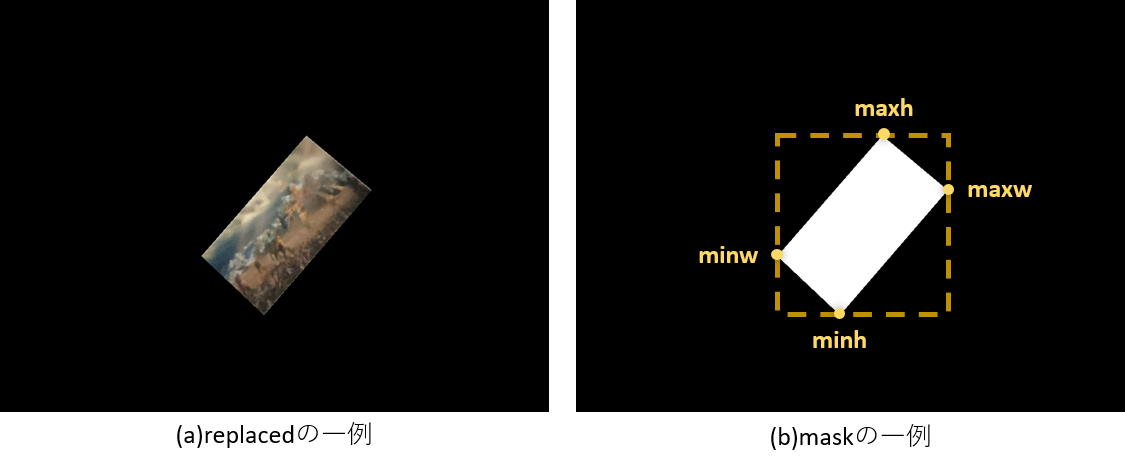
\includegraphics[width=1\linewidth]{fig/mask.png}
    \caption{探索領域の限定}
    \label{fig:mask}
\end{figure}

図\ref{fig:mask}(a)のようにreplacedは差し替え先画像の変換先以外がマスクされた画像となっている。
また、(b)のようにmaskは差し替え先画像が存在している領域を切り出す処理をしており、
後の探索領域の指定、すなわち、minh、minw、maxh、maxwの設定に利用する。

